\section{Overall \ac{REACT}  Framework}
\label{sec:framework}
\ac{REACT} framework, as depicted in \ref{fig:abstract}, consists of two main components: an offline planning phase and an online execution phase. In the offline phase, the environment is provided as a point cloud, including the object to be inspected. Then, a \ac{SDF} map is generated from this point cloud using the nvblox library \cite{nvblox}. Subsequently, the extracted point cloud of the structure under inspection is processed via FC-Planner \cite{feng2024fc} to compute an optimal waypoint sequence, generating a path that renders full inspection coverage while disregarding the tether constraints.

%Online Phase
In the online phase, tether constraints are handled by an entanglement-aware replanner that ensures that the maximum tether length is not exceeded due to entanglement. This is achieved using our developed tether model, which continuously updates based on the current state of the tether and the new position of the \ac{ROV}, denoted as $\textbf{p}_{\mathrm{rov}}$. The online planner then provides the reference state to an \ac{MPC} controller, which computes and applies the optimal wrench (forces and torques) to the \ac{ROV}.



%%%%%%%%%%%%%%%%%%%%%
%%%%%%  Tether Figure  
%%%%%%%%%%%%%%%%%%%%%

\begin{figure*}[t!]
    \centering
    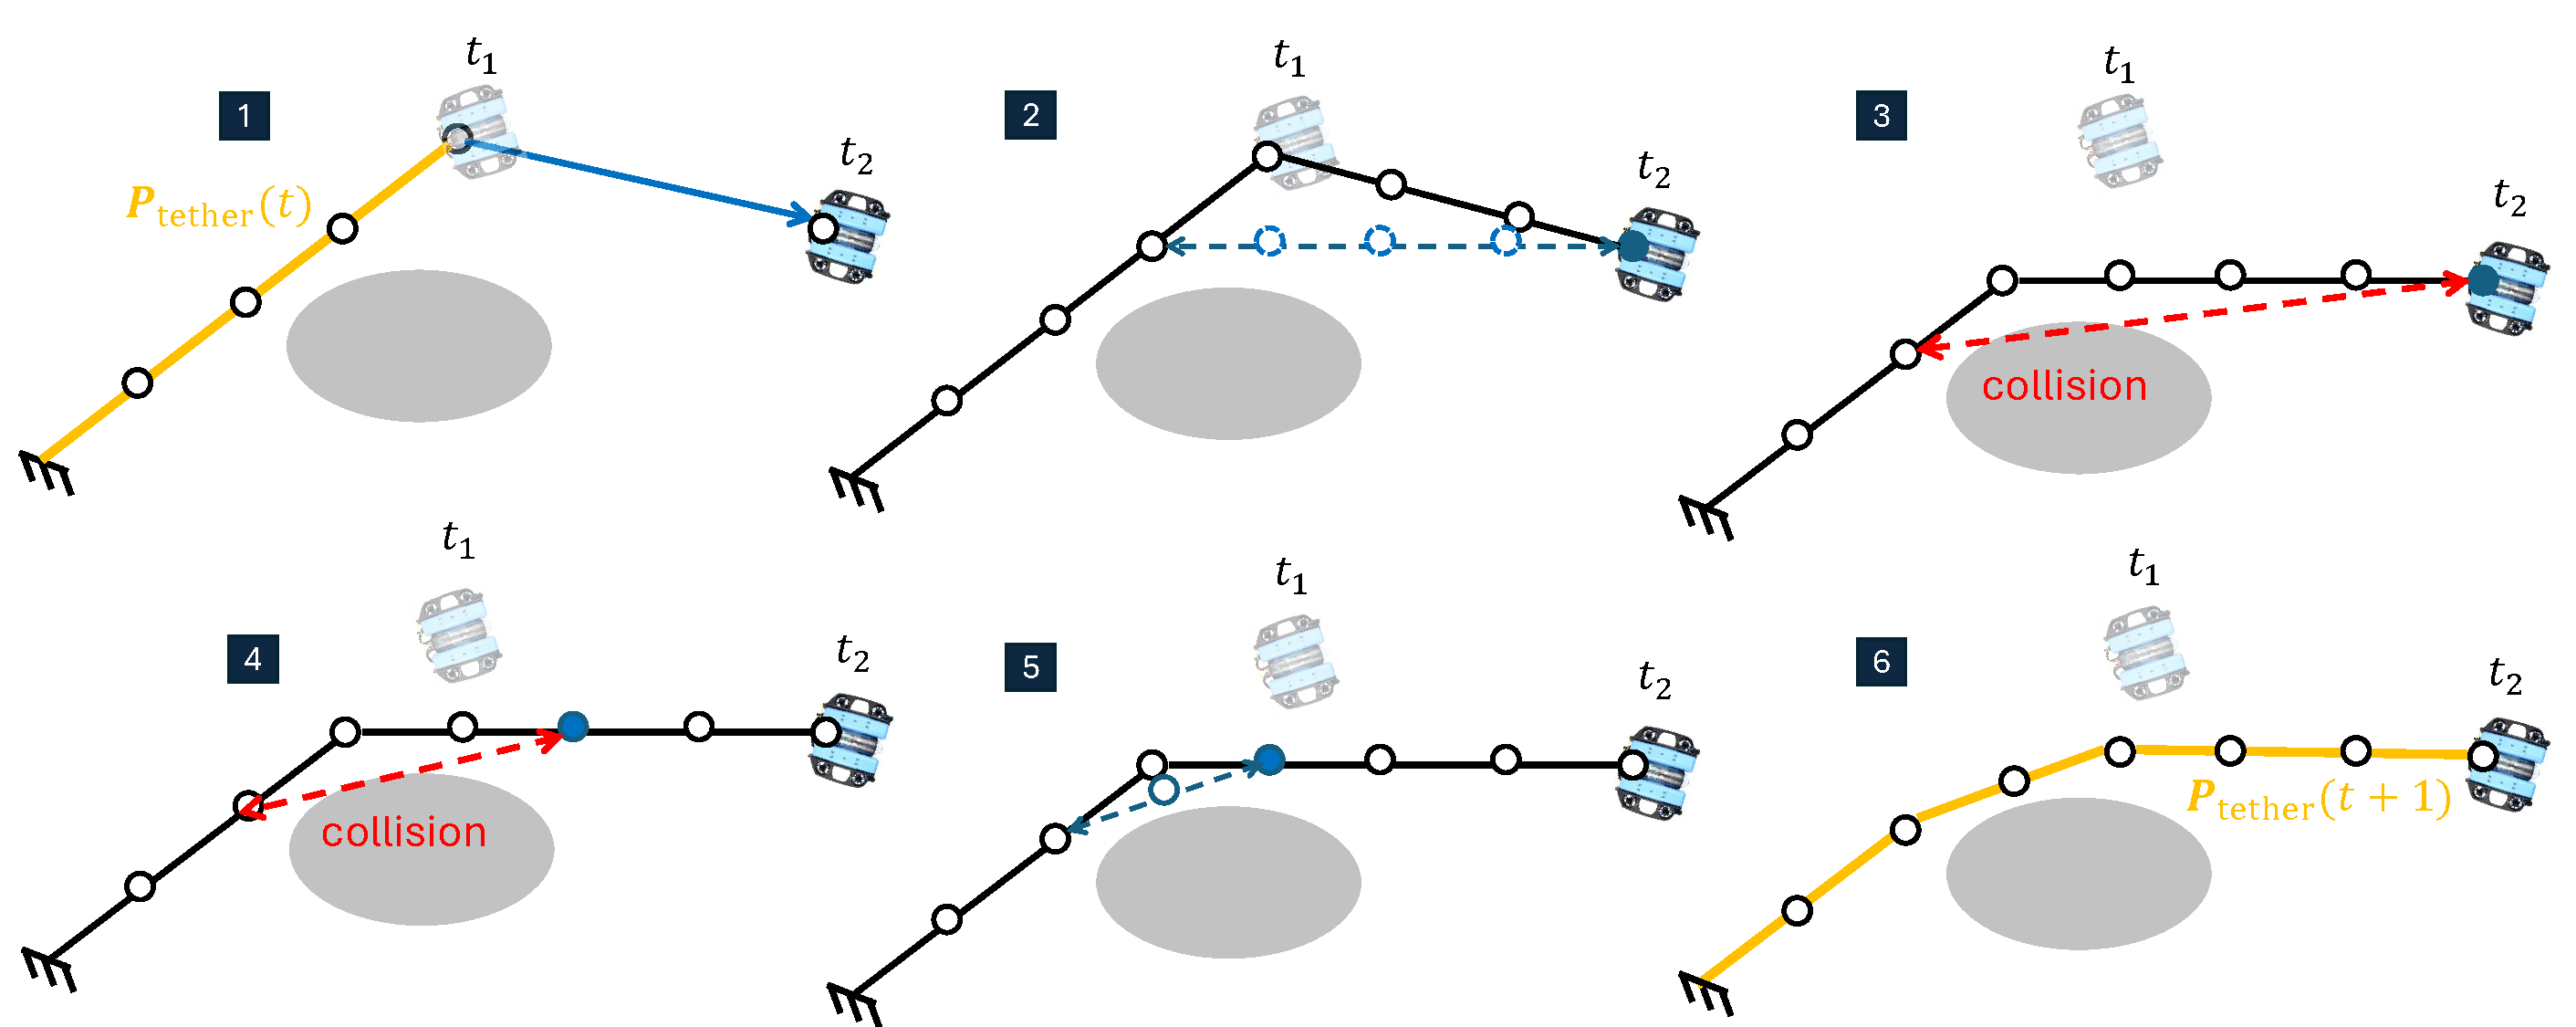
\includegraphics[width=1\linewidth]{EA-Planner/figures/tether_model.pdf}
    \caption{Tether shortcutting during \ac{ROV} motion from \( t_1 \) to \( t_2 \). (1) Initial tether with new \ac{ROV} position \( \mathbf{p}_{\text{rov}} \) appended; (2) Successful shortcut from the end node; (3) Collision encountered when attempting further shortcutting, skipping to the next node; (4) Another collision detected from the new node; (5) Successful shortcut from a subsequent node; (6) Final tether configuration (yellow) after applying all feasible shortcuts.}
    \label{fig:tether}
\end{figure*}
%%%%%%%%%%%%%%%%%%%%%%%%



%%%%%%%%%%%%%%%%%%%%%%%%%%%
%%%%%%%%%%%%%%%%%%%%%%%%%%%
%%%%%% Tether Model Section
%%%%%%%%%%%%%%%%%%%%%%%%%%%
%%%%%%%%%%%%%%%%%%%%%%%%%%%
\section{Tether Modeling}
\label{sec:tether_model}
%Next, we introduce a computationally efficient kinematic \ac{ROV} tether model, inspired by the shortcutting algorithm used in the ropeRRT path planner \cite{roperrt}. In essence, the proposed model predicts the position of each node along the tether length based on \ac{ROV}'s relative pose to the base. 
%which simplifies sampled trajectories in a manner analogous to a rope tightening around an obstacle. The key assumption in the proposed model is that we assume a geometry-based constraint where the tether remains taut and fully stretched at all times.

 We introduce a computationally efficient kinematic tether model for tethered underwater vehicles. This model predicts the tether path, specifically the positions of each node along the tether's length, based on the \ac{ROV}'s relative pose to the base, and assumes a geometry-based constraint where the tether remains taut and fully stretched at all times. The main idea of the proposed tether model is inspired by the shortcutting algorithm of the ropeRRT path planner \cite{roperrt}, which simplifies sampled trajectories similar to a rope tightening around an obstacle. 


\subsection{Tether model description}
Let the tether path at time \( t \) be denoted by \( \mathbf{P}_{\mathrm{tether}}(t) = \{ \mathbf{p}_i(t) \}_{i=1}^{N} \), where each node \( \mathbf{p}_i(t) \in \mathbb{R}^3 \) represents the position of the \( i \)-th node in 3D space at time \( t \), and \( N \) is the total number of nodes in the tether path. The \ac{ROV} position at time \( t \), denoted by \( \mathbf{p}_{\mathrm{rov}}(t) \in \mathbb{R}^3 \), is appended at the end \( \mathbf{p}_{N+1}(t) \), ensuring that the \ac{ROV}'s position is included in the tether path. 

The proposed tether model iteratively optimizes the tether path via two primary mechanisms: shortcutting and pulling. %, as illustrated in Fig.~\ref{fig:tether}. 
%For each pair of nodes \( (\mathbf{p}_i(t), \mathbf{p}_j(t)) \) where \( i < j \), the algorithm attempts to shortcut the path segment between them.
Starting at the last node ($\mathbf{p}_j(t) = \mathbf{p}_{N}(t)$), the algorithm attempts to shortcut the path segment between each pair of nodes \( (\mathbf{p}_i(t), \mathbf{p}_j(t)) \) where \( i < j \).
If the line of sight between \( \mathbf{p}_i(t) \) and \( \mathbf{p}_j(t) \) is collision-free, as determined via an \ac{SDF} map (\( \mathcal{M}_{sdf} \)), the intermediate nodes are replaced with a straight segment sampled at known resolution \( \delta_n \). Conversely, if the line of sight encounters a collision, $j$ shifts to the preceding node, and the collision-free line of sight is rechecked. This process is repeated until a collision-free line of sight is found, and the intermediate nodes are then replaced. Fig.~\ref{fig:tether} illustrates an example of the shortcut operation. 

Finally, after the shortcutting step, a pulling operation is applied to each node, moving it incrementally toward the tether endpoint \( \mathbf{p}_{N+1}(t) \). This ensures that nodes are not left stuck in cavities or grooves caused by non-convex obstacle shapes. The shortcutting and pulling operations are applied iteratively until convergence, resulting in a taut and collision-free tether path \( \mathbf{P}_{\mathrm{tether}}(t+1) \). The full procedure is described in Algorithm~\ref{alg:tether_optimization}.







%%%%%%%%%%%%%%%%%%%%%%%%%%%%%%%%%%%%%%%%%%
%%%%%%  Tether Model Algorithm  %%%%%%%%%
%%%%%%%%%%%%%%%%%%%%%%%%%%%%%%%%%%%%%%%%%%


\begin{algorithm}[t]
%\SetAlgoLined
\LinesNotNumbered  % Disable line numbers

\SetKwInOut{Input}{Require}
\SetKwInOut{Output}{Return}
\Input{
ROV position $\mathbf{p}_{\mathrm{rov}}(t)$, 
Tether path $\mathbf{P}_{\mathrm{tether}}(t)$, 
SDF map $\mathcal{M}_{sdf}$, 
parameters: $\delta_{n}$
}
\Output{Taut-tether at $t+1$ : $\mathbf{P}_{\mathrm{tether}}(t+1)$}
\BlankLine

\tcp{Extend tether path to include the current ROV position as the endpoint}
Append $\mathbf{p}_{\mathrm{rov}}(t)$ to $\mathbf{P}_{\mathrm{tether}}(t).end()$\;

%\tcp{Iterative shortcutting path segments by skipping intermediate nodes}
\tcp{Iterative shortcutting}
\For{$i \gets \mathrm{len}(\mathbf{P}_{\mathrm{tether}}(t)) - 1$ \textbf{to} $0$}{
    \For{$j \gets i - 1$ \textbf{to} $0$}{
        \tcp{Check if shortcutting the path is valid between nodes $i$ and $j$}
        \If{$\mathrm{checkShortcut}$($\mathbf{P}_{\mathrm{tether}}(t), i, j$)}{
            \tcp{Replace intermediate nodes $i-j$ }
            replaceNodes($\mathbf{P}_{\mathrm{tether}}(t)$, $i$, $j$, $\delta_{n}$)\;
        }
        \Else{
            \If{not $\mathrm{checkLineOfSight}$
            ($\mathcal{M}_{sdf}$, $\mathbf{P}_{\mathrm{tether}}(t)$)}{
                \tcp{Line of sight is blocked by obstacle, stop shortcutting}
                \textbf{break}\;
            }
            \If{$\mathrm{isInCollision}$($\mathcal{M}_{sdf}$, $\mathbf{P}_{\mathrm{tether}}(t)[j]$)}{
                \tcp{Pull node towards tether end}
                pullNode($\mathbf{P}_{\mathrm{tether}}(t)[j]$, $\mathbf{P}_{\mathrm{tether}}(t).end()$, $\delta_{n}$)\;
            }
        }
    }
}
\Return{$\mathbf{P}_{\mathrm{tether}}(t+1)$}\;
\caption{Taut-Tether Model}
\label{alg:tether_optimization}
\end{algorithm}




%%%%%%%%%%%%%%%%%%%%%%%%%%%
%%%%%%%%%%%%%%%%%%%%%%%%%%%
% Homotopy equivelance proof
%%%%%%%%%%%%%%%%%%%%%%%%%%%
%%%%%%%%%%%%%%%%%%%%%%%%%%%


% \subsection{Homotopic Equivalence of the Shortcutting-Based Tether Path}
% \label{sec:homotopy_proof}

% In this subsection, we demonstrate that the taut-tether path generated primarily through the shortcutting mechanism is homotopically equivalent to the Remotely Operated Vehicle's (ROV) actual trajectory. This argument focuses on the geometric simplification provided by shortcutting, assuming the tether behaves like a rope tightening around obstacles.

% \subsubsection{Preliminaries and Definitions}
% Let the ambient Euclidean space be $X = \mathbb{R}^3$. The static obstacle region, $O \subset X$, is a closed set. The \textbf{free configuration space} is defined as $C_{free} = X \setminus O$. A \textbf{path} in $C_{free}$ is a continuous function $\gamma: [0,1] \to C_{free}$.

% Two paths $\gamma_0, \gamma_1: [0,1] \to C_{free}$ sharing the same endpoints (i.e., $\gamma_0(0)=\gamma_1(0)$ and $\gamma_0(1)=\gamma_1(1)$) are said to be \textbf{homotopic in $C_{free}$} (denoted $\gamma_0 \sim \gamma_1$) if there exists a continuous function $H: [0,1] \times [0,1] \to C_{free}$, called a \textbf{homotopy}, such that:
% \begin{itemize}
%     \item $H(s,0) = \gamma_0(s)$ for all $s \in [0,1]$,
%     \item $H(s,1) = \gamma_1(s)$ for all $s \in [0,1]$,
%     \item $H(0,\tau) = \gamma_0(0)$ for all $\tau \in [0,1]$ (startpoints fixed),
%     \item $H(1,\tau) = \gamma_0(1)$ for all $\tau \in [0,1]$ (endpoints fixed).
% \end{itemize}
% Let $p_A \in C_{free}$ denote the fixed anchor point of the tether and $p_R(t) \in C_{free}$ be the ROV's position at time $t$. The actual continuous trajectory of the ROV up to time $t$ is a path $\Gamma_{\mathrm{rov}}: [0,1] \to C_{free}$, with $\Gamma_{\mathrm{rov}}(0) = p_A$ (assuming the path starts at the anchor for simplicity) and $\Gamma_{\mathrm{rov}}(1) = p_R(t)$.

% A \textbf{piecewise linear (PL) path}, $\mathbf{P}$, connecting $p_A$ to $p_R(t)$ is defined by an ordered sequence of $N+1$ vertices $(v_0, v_1, \ldots, v_N)$ where $v_0=p_A$, $v_N=p_R(t)$, and each $v_k \in C_{free}$. The path consists of line segments $L(v_k, v_{k+1}) = \{ (1-s)v_k + s v_{k+1} \mid s \in [0,1] \}$. For $\mathbf{P}$ to be a path in $C_{free}$, each segment $L(v_k, v_{k+1})$ must be entirely contained in $C_{free}$.

% \subsubsection{Initial Tether Path and Shortcutting as a Homotopy}
% Let $\mathbf{P}_{init}(t)$ be an initial PL path representing the tether before shortcutting optimization at time $t$. This path connects $p_A$ to $p_R(t)$ and is assumed to be a PL approximation of $\Gamma_{\mathrm{rov}}$ lying in $C_{free}$. It is a standard result in algebraic topology that $\Gamma_{\mathrm{rov}} \sim \mathbf{P}_{init}(t)$ if $\mathbf{P}_{init}(t)$ is a sufficiently fine approximation.

% The shortcutting mechanism iteratively refines a PL path. Let $\mathbf{P}_{k} = (v_0, \ldots, v_M)$ be the PL tether path at iteration $k$. A shortcutting step selects two non-consecutive vertices $v_i, v_j \in \mathbf{P}_{k}$ (where $i < j-1$). Let $\sigma_{old}$ be the subpath of $\mathbf{P}_{k}$ from $v_i$ to $v_j$, and let $\sigma_{new}$ be the straight-line segment $L(v_i, v_j)$. If $\sigma_{new} \subset C_{free}$ (i.e., the line of sight is collision-free), the path $\mathbf{P}_{k+1}$ is formed by replacing $\sigma_{old}$ with $\sigma_{new}$.

% \textbf{Claim:} If $\sigma_{new} \subset C_{free}$, then $\sigma_{old} \sim \sigma_{new}$ in $C_{free}$ relative to their common endpoints $v_i$ and $v_j$.

% \textit{Proof of Claim:}
% The tether model is "analogous to a rope tightening around an obstacle." When a flexible rope segment, initially following $\sigma_{old} \subset C_{free}$, is pulled taut between $v_i$ and $v_j$, and the direct path $\sigma_{new}$ is also in $C_{free}$, the rope physically deforms into $\sigma_{new}$ by moving exclusively through $C_{free}$.
% This continuous deformation can be represented by a homotopy. Let $\sigma_{old}(s)$ parameterize the PL path $\sigma_{old}$ for $s \in [0,1]$, and $\sigma_{new}(s) = (1-s)v_i + s v_j$ parameterize the segment $\sigma_{new}$. A straight-line homotopy is $H(s, \tau) = (1-\tau)\sigma_{old}(s) + \tau\sigma_{new}(s)$ for $s, \tau \in [0,1]$.
% The "rope tightening" analogy implies that if $\sigma_{new} \subset C_{free}$, then the entire region swept by the deformation from $\sigma_{old}$ to $\sigma_{new}$ is also contained in $C_{free}$. Thus, $H(s, \tau) \in C_{free}$ for all $s, \tau$. This ensures that $\sigma_{old} \sim \sigma_{new}$ in $C_{free}$.
% Since $\mathbf{P}_{k+1}$ is obtained from $\mathbf{P}_{k}$ by substituting $\sigma_{old}$ with a homotopic segment $\sigma_{new}$, it follows that $\mathbf{P}_{k} \sim \mathbf{P}_{k+1}$.
% \hfill $\qed$

% \subsubsection{Iterative Application and Final Equivalence}
% The shortcutting algorithm generates a sequence of PL paths $\mathbf{P}_{init}(t) = \mathbf{P}_0, \mathbf{P}_1, \ldots, \mathbf{P}_{final}$, where $\mathbf{P}_{final}$ is the resulting taut-tether path, denoted $\mathbf{P}^{tether}(t)$. Since each step is a homotopy, $\mathbf{P}_0 \sim \mathbf{P}_1 \sim \ldots \sim \mathbf{P}_{final}$. By the transitivity of the homotopy relation, $\mathbf{P}_{init}(t) \sim \mathbf{P}^{tether}(t)$.

% Given that $\Gamma_{\mathrm{rov}} \sim \mathbf{P}_{init}(t)$, and $\mathbf{P}_{init}(t) \sim \mathbf{P}^{tether}(t)$, we conclude by transitivity that:
% $$ \Gamma_{\mathrm{rov}} \sim \mathbf{P}^{tether}(t) $$
% Thus, the taut-tether path $\mathbf{P}^{tether}(t)$, resulting from the shortcutting operations, is homotopically equivalent to the ROV's actual trajectory $\Gamma_{\mathrm{rov}}$ within the free configuration space $C_{free}$. The shortcutting process simplifies the path to a tighter representative within its original homotopy class with respect to the obstacles.



%%%%%%%%%%%%%%%%%%%%%%%%%%%%%%%%%%%%%%%%%%
%%%%%%%%%%%%%%%%%%%%%%%%%%%%%%%%%%%%%%%%%%
%%%%%%%%%%%%%%%%%%%%%%%%%%%%%%%%%%%%%%%%%%



%%%%%%%%%%%%%%%%%%%%%%%%%%%
%%%%% REACT Planner %%%%%%
%%%%%%%%%%%%%%%%%%%%%%%%%%%
% \begin{algorithm}[t]
% \LinesNotNumbered  % Disable line numbers

% \SetKwInOut{Input}{Input}
% \SetKwInOut{Output}{Return}
% \Input{
% Waypoints $\mathbf{W}$, 
% Maximum tether length $L_{\max}$, 
% Current tether path $\mathbf{P}_{\mathrm{tether}}(t)$, 
% Current ROV position $\mathbf{p}_{\text{rov}}(t)$, 
% Current waypoint index $k$, $d_{\mathrm{thresh}}$}

% \Output{Target waypoint for the controller $\mathbf{p}_{\text{target}}$}
% \BlankLine

% Compute $L_{\text{tether}}(t)$ 

% \If{$L_{\mathrm{tether}}(t) > L_{\max}$ \textbf{and not} $search\_safe\_path$}{
%     $search\_safe\_path \gets$ True\; \tcp{Activate recovery mode}
%     $\mathbf{P}_{\text{recovery}} \gets \text{searchAlternativePath}(\mathbf{P}_{\mathrm{tether}}(t), \mathbf{W}[k], L_{\max})$\; \tcp{Find path within tether limits}
%     $\mathbf{P}_{\text{safe}} \gets \text{refineRecoveryPath}(\mathbf{P}_{\text{recovery}})$\; \tcp{Optimize the recovery path}
%     $is\_path\_safe$ $\gets \text{checkPathValidity}(\mathbf{P}_{\text{safe}})$\; \tcp{Check if recovery path is valid}
%     $safe\_path\_index$ $\gets 0$\; \tcp{Start from the beginning of the recovery path}
% }

% \If{$search\_safe\_path$ \textbf{and} $is\_path\_safe$}{
%     $\mathbf{p}_{\text{target}} \gets \text{getPointAlongPath}(\mathbf{P}_{\text{safe}}, \; safe\_path\_index)$\; \tcp{Get target from recovery path}
%     \If{$\|\mathbf{p}_{\mathrm{rov}}(t) - \mathbf{p}_{\mathrm{target}}\| < d_{\mathrm{thresh}}$}{
%         $safe\_path\_index \gets safe\_path\_index + 1$\; \tcp{Advance to next point}
%     }
%     \If{$safe\_path\_index \ge |\mathbf{P}_{\text{safe}}|$}{
%         $search\_safe\_path \gets$ False\; \tcp{Recovery complete}
%         $\mathbf{p}_{\text{target}} \gets \mathbf{W}[k]$\; \tcp{Resume wp tracking}
%     }
% }
% % hey sorry mohit, i didnt realize you were editing this
% \Else{
%     $search\_safe\_path \gets$ False\; \tcp{Reset recovery}
%     $\mathbf{p}_{\mathrm{target}} \gets \mathbf{W}[k]$\; \tcp{Default to current wp}

%     \If{$\|\mathbf{p}_{\mathrm{rov}}(t) - \mathbf{p}_{\mathrm{target}}\| < d_{\mathrm{thresh}}$}{
%          $k \gets k + 1$\; \tcp{Advance to next wp}
%     }
% }
% \Return{$\mathbf{p}_{\mathrm{target}}$}\;
% \caption{Real-time Entanglement-Aware Path Planning}
% \label{alg:main_loop}
% \end{algorithm}










%%%%%%%%%%%%%%%%%%%%%%%%%%%%%%%%%
%% Alg. 3 Recovery Path  Algorithm %%%
%%%%%%%%%%%%%%%%%%%%%%%%%%%%%%%%%

% \begin{algorithm}[b]
% \LinesNotNumbered  % Disable line numbers
% \SetKwInOut{Input}{Input}
% \SetKwInOut{Output}{Return}
% \Input{
% Current tether $\mathbf{P}(t)$,
% Goal waypoint $\mathbf{p}_{\text{goal}}$,
% Maximum length $L_{\max}$
% }
% \Output{Recovery path segment $\mathbf{P}_{\text{recovery}}$}
% \BlankLine
%  $best\_path$ $\gets$ None\; \\
%  $prev\_len$ $\gets \infty$\; \\
%  $found\_suitable$ $\gets$ False\; \\
% \For{$i \gets |\mathbf{P}(t)| - 3$ \textbf{downto} 3}{
%     $\mathbf{P}_{\text{candidate}} \gets \text{generatePath}(i, \mathbf{P}(t), \mathbf{p}_{\text{goal}})$\; \\
%     $L_{\text{candidate}} \gets \text{computeLength}(i, \mathbf{P}(t), \mathbf{P}_{\text{candidate}})$\;\\
%     \If{$L_{\text{candidate}} < 0.7L_{\max}$} %\textbf{and} $L_{\text{candidate}} < 0.65 \cdot \text{prev\_len}$}
%     {
%           $best\_path$ $\gets \text{ExtractSegment}(i+2, \mathbf{P}(t))$\;
%          found\_suitable $\gets$ True\;
%          \textbf{break}\;
%     }
%      $prev\_len$ $\gets \text{computeLength}(i-3, \mathbf{P}(t), \text{generatePath}(i-3, \mathbf{P}(t), \mathbf{p}_{\text{goal}}))$\;
% }
% \If{\textbf{not} found\_suitable}{
%     $\mathbf{p}_{\text{rov}} \gets \mathbf{P}(t)[|\mathbf{P}(t)|-1]$\; \tcp{Fallback}
%     $\mathbf{P}_{\text{recovery}}$ $\gets \text{planShortestPath}(\mathbf{p}_{\text{rov}}, \mathbf{p}_{\text{goal}})$\;
% }
% \Return{$\mathbf{P}_{\text{recovery}}$}\;
% \caption{Search Alternative Recovery Path}
% \label{alg:search_alternative}
% \end{algorithm}

%%%%%%%%%%%%%%%%%%%%%%%%%%%%%%%%%%%%%%%%%%
%%%%%%%%%%%%%%%%%%%%%%%%%%%%%%%%%%%%%%%%%%
%%%%%%%%%%%%%%%%%%%%%%%%%%%%%%%%%%%%%%%%%%

%%%%%%%%%%%%%%%%%%%%%%%%%%%
%%%%% REACT Planner %%%%%%
%%%%%%%%%%%%%%%%%%%%%%%%%%%






%%%%%%%%%%%%%%%%%%%%%%%%%%%%%%%%%
%% Alg. 3 Recovery Path Algorithm %%%
%%%%%%%%%%%%%%%%%%%%%%%%%%%%%%%%%
% \begin{algorithm}[t]
% \LinesNotNumbered  % Disable line numbers
% \SetKwInOut{Input}{Input}
% \SetKwInOut{Output}{Output}
% \Input{
% Current tether $\mathbf{P}_{\text{tether}}(t)$,
% Target waypoint $\mathbf{W}[k]$,
% Maximum length $L_{\max}$
% }
% \Output{Recovery path $\mathbf{P}_{\text{recovery}}$ with segments $\mathbf{P}_{\text{r}1}$ and $\mathbf{P}_{\text{r}2}$}
% \BlankLine
%  $\mathbf{p}_{\text{pivot}} \gets$ None\; \\
%  $found\_feasible$ $\gets$ False\; \\
%  \BlankLine
%  \tcp{Backward recovery search along tether trajectory}
% \For{$i \gets |\mathbf{P}_{\text{tether}}(t)| - 2$ \textbf{downto} 1}{
%     $\mathbf{p}_{\text{candidate}} \gets \mathbf{P}_{\text{tether}}(t)[i]$\; \\
%     $\mathbf{P}_{\text{c}} \gets \text{planShortestPath}(\mathbf{p}_{\text{candidate}}, \mathbf{W}[k])$\; \\
%     \BlankLine
%     \tcp{Create candidate path and simulate tether using tether model}
%     $\mathbf{P}_{\text{candidate\_path}} \gets \text{extractSegment}(0, i, \mathbf{P}_{\text{tether}}(t)) \cup \mathbf{P}_{\text{c}}$\; \\
%     $\mathbf{P}_{\text{tether}}(t+1) \gets \text{tetherModel}(\mathbf{P}_{\text{candidate\_path}})$\; \\
%     $L_{\text{new}} \gets \text{computeLength}(\mathbf{P}_{\text{tether}}(t+1))$\; \\
%     \BlankLine
%     \If{$L_{\text{new}} \leq L_{\max}$}{
%         $\mathbf{p}_{\text{pivot}} \gets \mathbf{p}_{\text{candidate}}$\; \\
%         $\mathbf{P}_{\text{r}1} \gets \text{extractSegment}(0, i, \mathbf{P}_{\text{tether}}(t))$\; \\
%         $\mathbf{P}_{\text{r}2} \gets \mathbf{P}_{\text{c}}$\; \\
%         $found\_feasible \gets$ True\;
%         \textbf{break}\;
%     }
% }
% \BlankLine
% \If{\textbf{not} found\_feasible}{
%     \tcp{Fallback: treat tether constraint as soft constraint}
%     $\mathbf{p}_{\text{pivot}} \gets \mathbf{p}_{\text{rov}}(t)$\; \tcp{Current ROV position}
%     $\mathbf{P}_{\text{r}1} \gets \emptyset$\; \\
%     $\mathbf{P}_{\text{r}2} \gets \text{planShortestPath}(\mathbf{p}_{\text{pivot}}, \mathbf{W}[k])$\;
% }
% \BlankLine
% $\mathbf{P}_{\text{recovery}} \gets \mathbf{P}_{\text{r}1} \cup \mathbf{P}_{\text{r}2}$\;
% \Return{$\mathbf{P}_{\text{recovery}}$}\;
% \caption{De-entanglement Path Search}
% \label{alg:search_alternative}
% \end{algorithm}





%%%%%%%%%%%%%%%%%%%%%%%%%%%
%% Refine Path  Algorithm
%%%%%%%%%%%%%%%%%%%%%%%%%%%
% \begin{algorithm}[t]
% \LinesNotNumbered  % Disable line numbers
% \SetKwInOut{Input}{Input}
% \SetKwInOut{Output}{Return}
% \Input{
%     Recovery path $\mathbf{P}_{\text{recovery}}$;\\
%     Offset distance $\delta_{\text{offset}}$;\\
%     Sampling distance $\delta_{\text{sample}}$
% }
% \Output{Refined safe path $\mathbf{P}_{\text{safe}}$}
% \BlankLine
% $\mathbf{P}_{\text{offset}} \gets \text{tetherPathOffset}(\mathbf{P}_{\text{recovery}}, \delta_{\text{offset}})$\;
% \\
% $\mathbf{P}_{\text{sampled}} \gets \text{perturbTetherPath}(\mathbf{P}_{\text{offset}}, \delta_{\text{sample}})$\;
% \\
% $\mathbf{P}_{\text{safe}} \gets \text{smoothTetherPath}(\mathbf{P}_{\text{sampled}})$\;
% \\
% \Return{$\mathbf{P}_{\text{safe}}$}\;
% \caption{Refine Recovery Path}
% \label{alg:refine_path}
% \end{algorithm}


%%%%%%%%%%%%%%
%%%%%%%%%%%%%%
%%%%%%%%%%%%%%

%%%%%%%%%%%%%%%%%%%%%%%%%%%
%%%%%%%%%%%%%%%%%%%%%%%%%%%
%%%%%%% PLANNER %%%%%%%%%
%%%%%%%%%%%%%%%%%%%%%%%%%%
%%%%%%%%%%%%%%%%%%%%%%%%%%





\section{Entanglement-Aware Path Planner}
\label{sec:planner}


Next, we present the entanglement-aware path planner, a local planner designed to address the real-time entanglement avoidance problem for tethered underwater vehicles. The planner continuously monitors the tether configuration and dynamically adjusts the vehicle’s target to prevent the tether length from exceeding a specified maximum allowable length, \( L_{\max} \), while ensuring safe navigation toward a series of predefined reference waypoints.

At each time step \( t \), the planner receives the current estimated tether path, \(\mathbf{P}_{\mathrm{tether}}(t)\), from the tether model. It also maintains an ordered list of target waypoints, \(\mathbf{W} = \{\mathbf{p}_{\text{waypoint}}(k)\}_{k=1}^M\), where each \(\mathbf{p}_{\text{waypoint}}(k)\) specifies a 3D position the ROV must reach sequentially. The current position of the ROV, \(\mathbf{p}_{\text{rov}}(t)\), and the current waypoint index, \(k\), are also maintained as part of the planner’s state.

The current tether length \(L_{\text{tether}}(t)\) is computed from the tether path and compared against the maximum allowable tether length \(L_{\max}\) to determine whether re-planning is necessary.

If the tether length exceeds the limit, i.e., \( L_{\text{tether}}(t) > L_{\max} \), the planner switches to a \emph{de-entanglement} mode. In this mode, a recovery path is generated by searching for an alternative safe path toward the current waypoint that respects the tether constraints and reduces the risk of entanglement. The ROV’s target position is then updated to incrementally follow this recovery path.

If the tether length remains within the allowable limit, the planner operates in nominal mode. It sets the target position directly to the current waypoint. Upon detecting that the ROV has reached this waypoint, the planner advances the waypoint index \(k\) to progress to the next target in the sequence.

This approach ensures that the vehicle maintains a safe tether configuration while effectively progressing through its mission waypoints. The planner continuously switches between nominal waypoint tracking and recovery behaviors in response to tether length measurements, enabling real-time, entanglement-aware path planning.



%%%%%%%%%%%%%%%%%%%%%%%%%%%
%%%%% REACT Planner %%%%%%
%%%%%%%%%%%%%%%%%%%%%%%%%%%
\begin{algorithm}[t]
\LinesNotNumbered  % Disable line numbers
\SetKwInOut{Input}{Input}
\SetKwInOut{Output}{Output}
\Input{
Waypoints $\mathbf{W}$, 
Maximum tether length $L_{\max}$, 
Current tether path $\mathbf{P}_{\mathrm{tether}}(t)$, 
Current ROV position $\mathbf{p}_{\text{rov}}(t)$, 
Current waypoint index $k$
}
\Output{Target position $\mathbf{p}_{\text{target}}$ for ROV controller}
\BlankLine
\tcp{Entanglement Detection}
$L_{\text{tether}}(t) \gets \text{computeLength}(\mathbf{P}_{\mathrm{tether}}(t))$\;
\BlankLine
\If{$L_{\mathrm{tether}}(t) > L_{\max}$}{
    \tcp{De-entanglement Mode: Search for recovery path}
    $\mathbf{P}_{\text{safe}} \gets \text{deEntanglementPathSearch}(\mathbf{P}_{\mathrm{tether}}(t), \mathbf{W}[k], L_{\max})$\;
    \BlankLine
    %\If{$\mathbf{P}_{\text{safe}}$ is valid}{
        $\mathbf{p}_{\text{target}} \gets \text{followRecoveryPath}(\mathbf{P}_{\text{safe}}, \mathbf{p}_{\text{rov}}(t))$\;
    }
%    \Else{
 %       $\mathbf{p}_{\text{target}} \gets \text{emergencyFallback}(\mathbf{p}_{\text{rov}}(t))$\; \tcp{wait}
 %   }
%}
\Else{
    \tcp{Normal Waypoint Following Mode}
    $\mathbf{p}_{\text{target}} \gets \mathbf{W}[k]$\;
    \BlankLine
    \If{ROV reached current waypoint}{
        $k \gets k + 1$\; \tcp{Advance to next waypoint}
    }
}
\BlankLine
\Return{$\mathbf{p}_{\text{target}}$}\;
\caption{Real-time Entanglement-Aware Path Planning}
\label{alg:main_loop}
\end{algorithm}




\subsection{De-entanglement path search}


To implement the de-entanglement behavior described above, the recovery path search algorithm (Algorithm~\ref{alg:search_alternative}) is employed. This algorithm takes as input the current tether path, represented as an ordered sequence of points \(\mathbf{P}_{\mathrm{tether}}(t)\) of length \(n\), the current target waypoint \(\mathbf{W}[k]\), and the maximum allowable tether length \(L_{\max}\). Its goal is to generate a recovery path \(\mathbf{P}_{\mathrm{recovery}}\) that guides the \ac{ROV} safely toward the waypoint while ensuring that the tether length constraint is respected.

The algorithm performs a backward search along the tether path, starting from the \ac{ROV}’s current position at the tether’s end and progressing toward its origin. At each iteration, a candidate pivot point \(\mathbf{p}_{\mathrm{pivot}}\) on the tether is selected as a potential point from which the \ac{ROV} can attempt an alternative route toward the target waypoint.

For each pivot, two path segments are constructed. The first segment, \(\mathbf{P}_{\mathrm{r}1}\), corresponds to the reversed portion of the tether from the pivot \(\mathbf{p}_{\mathrm{pivot}}\) to the \ac{ROV}’s current position, representing the retraced section of the tether. The second segment, \(\mathbf{P}_{\mathrm{s}(n - i)}\), is a newly planned shortest path connecting the pivot to the target waypoint \(\mathbf{W}[k]\), which can be computed using sampling-based methods such as RRT*. These segments are then concatenated with the tether path from the origin up to the pivot, forming an augmented candidate path \(\mathbf{P}_{\mathrm{aug}}\).

This candidate path \(\mathbf{P}_{\mathrm{aug}}\) is used to simulate the tether configuration and estimate its length \(L_{\mathrm{tether}}\) at the next time step. The total tether length \(L_{\mathrm{tether}}\) is then compared against the maximum allowable length \(L_{\max}\). If the length constraint is satisfied, the recovery path \(\mathbf{P}_{\mathrm{recovery}} = \mathbf{P}_{\mathrm{r}1} \cup \mathbf{P}_{\mathrm{s}(n - i)}\) is considered feasible and returned.

If no feasible path is found after examining all possible pivot points, the algorithm defaults to a fallback strategy where the tether length constraint is treated as a soft limit. In this case, the recovery path consists solely of the shortest path from the \ac{ROV}’s current position directly to the target waypoint, temporarily disregarding tether length constraints.

The resulting recovery path provides a safe and viable trajectory for the \ac{ROV} to follow during de-entanglement operations by combining the reversed tether segment (if applicable) with the newly planned path toward the waypoint, as illustrated in Figure~\ref{fig:planner_search}.










%%%%%%%%%%%%%%%%%%%%%%%%%%%%%%%%%
%% Alg. 3 Recovery Path Algorithm %%%
%%%%%%%%%%%%%%%%%%%%%%%%%%%%%%%%%
\begin{algorithm}[t]
\LinesNotNumbered  % Disable line numbers
\SetKwInOut{Input}{Input}
\SetKwInOut{Output}{Output}
\Input{
Tether path \( \mathbf{P}_{\text{tether}}(t) \) of length \( n \),\\
Target waypoint \( \mathbf{W}[k] \),\\
Maximum tether length \( L_{\max} \)
}
\Output{
Recovery path \( \mathbf{P}_{\text{recovery}} = \mathbf{P}_{\text{r}1} \cup \mathbf{P}_{\text{r}2} \)
}
\BlankLine
$found\_feasible \gets \textbf{False}$\;
\BlankLine
\tcp{Backward recovery search from current ROV position}
\For{$i \gets n - 1$ \textbf{downto} 0}{
    $\mathbf{p}_{\text{pivot}} \gets \mathbf{P}_{\text{tether}}(t)[i]$\;\\
    \tcp{Extract tether segment backward from end (ROV) to pivot and reverse it}
    $\mathbf{P}_{\text{r}1} \gets \text{reverseSegment}(i, n-1, \mathbf{P}_{\text{tether}}(t))$\; \\
    $\mathbf{P}_{\text{s}(n - i)} \gets \text{planShortestPath}(\mathbf{p}_{\text{pivot}}, \mathbf{W}[k])$\;
    \BlankLine
    \tcp{Simulate tether with segment up to pivot + shortest path}
    $\mathbf{P}_{\text{aug}} \gets \text{concatenate}(\mathbf{P}_{\text{tether}}(t)[0:i], \mathbf{P}_{\text{s}(n - i)})$\; \\
    $\mathbf{P}_{\text{tether}}(t+1) \gets \text{tetherModel}(\mathbf{P}_{\text{aug}})$\; \\
    $L_{\text{tether}} \gets \text{computeLength}(\mathbf{P}_{\text{tether}}(t+1))$\;
    \BlankLine
    \If{$L_{\text{tether}} \leq L_{\max}$}{
        $\mathbf{P}_{\text{r}2} \gets \mathbf{P}_{\text{s}(n - i)}$\;
        $found\_feasible \gets \textbf{True}$\;
        \textbf{break}\;
    }
}
\BlankLine
\If{\textbf{not} $found\_feasible$}{
    \tcp{Fallback: treat tether constraint as soft}
    $\mathbf{p}_{\text{pivot}} \gets \mathbf{P}_{\text{tether}}(t)[-1]$\; \\
    $\mathbf{P}_{\text{r}1} \gets \emptyset$\; \\
    $\mathbf{P}_{\text{r}2} \gets \text{planShortestPath}(\mathbf{p}_{\text{pivot}}, \mathbf{W}[k])$\;
}
\BlankLine
$\mathbf{P}_{\text{recovery}} \gets \mathbf{P}_{\text{r}1} \cup \mathbf{P}_{\text{r}2}$\;
\Return{$\mathbf{P}_{\text{recovery}}$}\;
\caption{De-entanglement Path Search}
\label{alg:search_alternative}
\end{algorithm}











%%%%%%%%%%%%%%%%%%%%%%%%%
%%%% Figure : Planner search 
%%%%%%%%%%%%%%%%%%%%%%%%
%%%%%%%%%%%%%%%%%%%%%%%%
% \begin{figure*}[h]
%     \centering
%     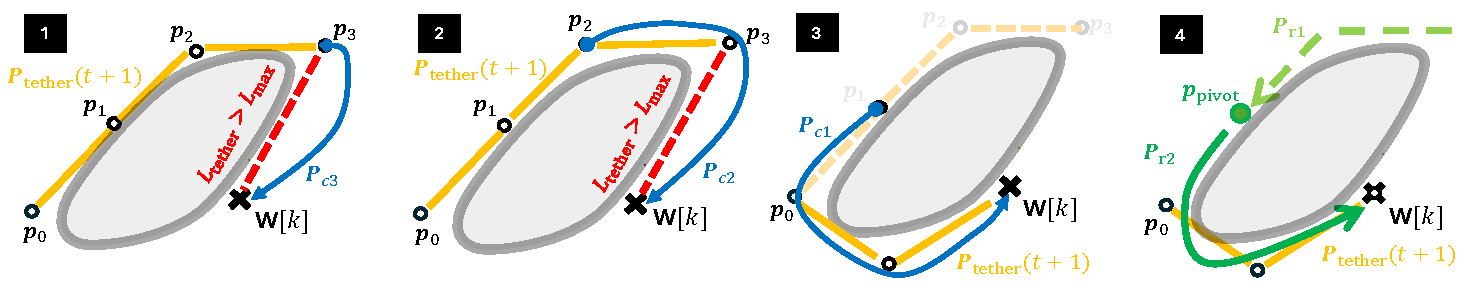
\includegraphics[width=\textwidth]{EA-Planner/figures/planner_newest.pdf}
%     \caption{De-entanglement path search process. 
%     (1) Entanglement detection: following the path from node \( \mathbf{p}_3 \), denoted as \( \mathbf{P}_{c_3} \), causes the tether length \( L_{\text{tether}} \) to exceed the maximum allowed length \( L_{\text{max}} \); 
%     (2) a backward recovery search is initiated from node \( \mathbf{p}_2 \) along the tether trajectory \( \mathbf{P}_{\mathrm{tether}}(t) \), but the resulting path yields no improvement in tether length; 
%     (3) continuing the search further back to node \( \mathbf{p}_1 \) leads to a feasible path and an updated, valid tether configuration; 
%     (4) the final planned safe path \( \mathbf{P}_{\text{safe}} \) (green), which satisfies the tether constraint (\( L_{\text{tether}} \leq L_{\text{max}} \)), consists of two segments: \( \mathbf{P}_{\text{safe},1} \), the part of the tether path up to node \( \mathbf{p}_1 \) (also \( \mathbf{p}_{\text{pivot}} \)), and \( \mathbf{P}_{\text{safe},2} \), the shortest path from \( \mathbf{p}_2 \) towards the target waypoint \( \mathbf{W}[k] \), ensuring an entanglement-free tether path $\mathbf{P}_{\mathrm{tether}}(t+1)$.}
%     \label{fig:planner_search}
% \end{figure*}
%%%%%%%%%%%%%%%%
%%%%%%%%%%%%%%%%
% \begin{figure*}[h]
%     \centering
%     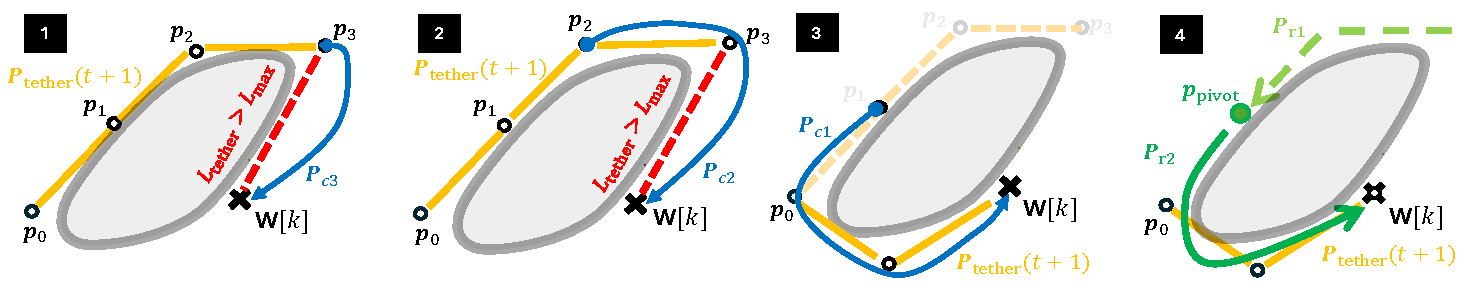
\includegraphics[width=\textwidth]{EA-Planner/figures/planner_newest.pdf}
%     \caption{De-entanglement path search process. 
%     (1) Entanglement detection: following the path from node \( \mathbf{p}_3 \), denoted as \( \mathbf{P}_{c_3} \), causes the tether length \( L_{\text{tether}} \) to exceed the maximum allowed length \( L_{\text{max}} \); 
%     (2) a backward recovery search is initiated from node \( \mathbf{p}_2 \) along the tether trajectory \( \mathbf{P}_{\mathrm{tether}}(t) \). The candidate path \( \mathbf{P}_{c_2} \) (tether segment to \( \mathbf{p}_2 \) plus shortest path to waypoint) is evaluated using the tether model, but the resulting simulated tether length yields no feasible solution; 
%     (3) continuing the search further back to node \( \mathbf{p}_1 \) leads to a feasible path. The candidate path \( \mathbf{P}_{c_1} \) produces a simulated tether configuration that satisfies the length constraint; 
%     (4) the final planned recovery path \( \mathbf{P}_{\text{recovery}} \) (green), which satisfies the tether constraint (\( L_{\text{tether}} \leq L_{\text{max}} \)), consists of two segments: \( \mathbf{P}_{\text{r}1} \), the part of the tether path up to node \( \mathbf{p}_1 \) (also \( \mathbf{p}_{\text{pivot}} \)), and \( \mathbf{P}_{\text{r}2} \), the shortest path from \( \mathbf{p}_1 \) towards the target waypoint \( \mathbf{W}[k] \), ensuring an entanglement-free tether path $\mathbf{P}_{\mathrm{tether}}(t+1)$.}
%     \label{fig:planner_search}
% \end{figure*}
\begin{figure*}[h]
    \centering
    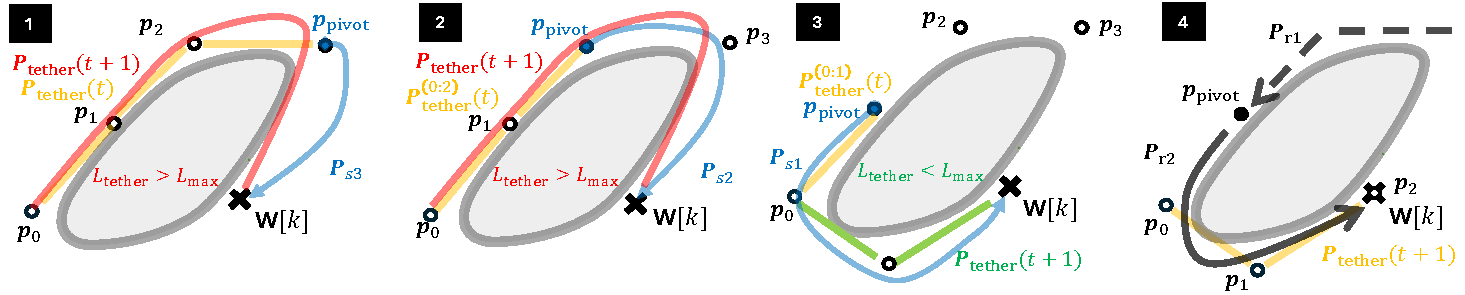
\includegraphics[width=\textwidth]{EA-Planner/figures/planner_newest1.pdf}
    \caption{De-entanglement path search process. At time \( t \), the tether configuration is \( \mathbf{P}_{\text{tether}}(t) = \{\mathbf{p}_0, \mathbf{p}_1, \mathbf{p}_2, \mathbf{p}_3\} \). 
    (1) The shortest path \( \mathbf{P}_{s3} \) from \( \mathbf{p}_3 \) to the waypoint \( \mathbf{W}[k] \) is appended to the tether path, forming the augmented path \( \mathbf{P}_{\text{tether}}^{(0:3)} \cup \mathbf{P}_{s3} \), which is passed to the tether model to compute \( \mathbf{P}_{\text{tether}}(t+1) \). The resulting tether length exceeds \( L_{\max} \), indicating a violation. 
    (2) The pivot shifts to \( \mathbf{p}_2 \), and the augmented path \( \mathbf{P}_{\text{tether}}^{(0:2)} \cup \mathbf{P}_{s2} \) is evaluated, but still violates the constraint. 
    (3) With pivot at \( \mathbf{p}_1 \), the augmented path \( \mathbf{P}_{\text{tether}}^{(0:1)} \cup \mathbf{P}_{s1} \) yields a feasible configuration with \( L_{\text{tether}} \leq L_{\max} \). 
    (4) The final recovery path \( \mathbf{P}_{\text{recovery}} \) consists of \( \mathbf{P}_{\text{r}1} \), tracing back from \( \mathbf{p}_3 \) to \( \mathbf{p}_1 \), and \( \mathbf{P}_{\text{r}2} = \mathbf{P}_{s1} \), leading to the waypoint \( \mathbf{W}[k] \).}
    \label{fig:planner_search}
\end{figure*}










\subsection{Recovery path refinement}
The initially selected recovery path \( \mathbf{P}_{\text{recovery}} \) undergoes further refinement to enhance safety and smoothness before execution. This involves several steps:
\begin{enumerate}
    \item Centroid Offsetting: Points along \( \mathbf{P}_{\text{recovery}} \) are pushed slightly outwards, away from the path's geometric centroid, to increase clearance from potential obstacles near the path's center.
    \item Random Sampling Perturbation: Points are locally perturbed by sampling in random directions, seeking nearby collision-free states to potentially escape minor constraint violations or local minima.
    \item Polynomial Smoothing: A third order polynomial function is fitted to segments of the path to reduce sharp turns and generate a smoother reference trajectory.
\end{enumerate}
The resulting refined path is denoted as \( \mathbf{P}_{\text{safe}} \). The planner then checks if \( \mathbf{P}_{\text{safe}} \) is collision-free. This refinement process is performed in a loop that continues until a collision-free path is found.















%%%%%%%%%%%%%%%%%%%%%%%%%%%%%%%%%%%%%%%%%%
%%%%%%%%%%%%%%%%%%%%%%%%%%%%%%%%%%%%%%%%%%
%%%%%%%%%%%%%%%%%%%%%%%%%%%%%%%%%%%%%%%%%%













